\chapter{\label{chap:implementierung}Implementierung der Prototypen}
In diesem Kaptitel wird nach dem in Kapitel \ref{chap:konzeption} präsentiertem Lösungsweg die detaillierte Beschreibung der technischen Realisierung der Prototypen vorgestellt.\\
Nach der Beschreibung der Realisierung der grundlegenden Funktionen der Anwendung wird auf die Umsetzung der Offlinefunktionalität und des Konfliktmanagements eingegangen.
Im Zuge dessen wird der implementierte Algorithmus zur Lösung auftretender Konflikte vorgestellt.
%
%
%
\section{Die Contacts Komponente}
Die Herzstück jeder zu entwickelnden Anwendung ist die Komponente \tt{Contacts}.
Sie beinhaltet die zentralen Funktionalitäten und entscheidet welche Anzeigeelemente gerendert werden und welche nicht.
Im Prototypen \it{amilia-qouch} besteht sie aus der Datei \tt{Contacts.js} in der ein interne State festgelegt ist. Hier sind außerdem Funktionen implementiert über die der State manipuliert werden kann.\\
Durch den in \autoref{chap:redux} beschriebenen, Redux--spezifischen Datenfluss ist sie auf mehrere Dateien aufgeteilt.
\tt{Contacts.js} ist für das Rendern der anderen Komponenten zuständig. 
In \tt{actions.js} werden die Aktionen definiert, die über die Containerkomponente \tt{ContactsContainer.js} von jeder Komponente aufgerufen werden können um den \gls{App}state zu manipulieren.
Die Manipulation wird in der \tt{reducer.js} behandelt, wo die geänderte Kopie wieder zurück an den \tt{Store} gegeben wird und sie wieder bei der \tt{Contacts.js} ankommt.
Der Einfachheit halber wird im Folgenden von der \tt{Contacts} Komponente geschrieben, wobei für den Redux Prototypen der Zusammenschluss dieser soeben beschriebenen Dateien gemeint ist.\\\\
Die Methode \tt{componentDidMount} ist die dritte im React Komponenten--Lebenszyklus\footnote{ \url{https://reactjs.org/docs/react-component.html\#the-component-lifecycle} -- Zugriff: 28.07.1018} und wird aufgerufen sobald die Anwendung gemountet ist.
Hier werden werden die Kontakte geladen und im \gls{App}state gespeichert.
Sobald sicht der \gls{App}state ändert wird die \tt{render} Funktion der Komponente aufgerufen. \autoref{code:render} zeigt die Renderfunktion der \tt{Contacts} Komponente.
%
\begin{center}
  \lstinputlisting[language=REACT,numbers=left,xleftmargin=20pt,framexleftmargin=15pt,
  caption={Die Renderfunktion der \tt{Contacts} Komponente des Prototypen \it{amilia-qouch}},
  label=code:render]{code/render.js}
\end{center}
%
Unabhängig von einem Wert im State wird der Header, in den Zeilen fünf bis sieben, gerendert.
Im wird die Information \tt{isOpen} übergeben die aussagt ob der Editiermodus an ist, also ob das Formular gerade geöffnet ist oder nicht.
Ihm wird auch die Funktion \tt{toggleEdit} gegeben, welche genau diese Statuseigenschaft wechselt.\\
Die Zeilen neun bis 14 gibt es nur im \it{amilia-qouch} Prototypen. Näheres dazu wird weiter unten im \autoref{chap:konfliktmanagement} erklärt.\\
In den Zeilen 16 bis 27 wird anhand der \tt{isOpen} Information entschieden ob das Formular oder die Liste gerendert wird.
Die Liste bekommt alle im \gls{App}state gespeicherten Kontakte, ebenfalls die \tt{toggleEdit} Funktion und eine zum Löschen eines Kontakt. Es ist zu beachten, dass hier bei der \tt{toggleEdit()} das \tt{bind(this, null)} fehlt. Das liegt daran, dass wenn man aus der Liste das Formular öffnet, man den 'Bearbeiten' Knopf betätigt hat und der zu bearbeitende Kontakt im Formular geladen wird. Dieser Kontakt wird dann für die Dauer seiner Bearbeitung im \tt{state.editView.contact} gespeichert.\\
Das KontaktFormular ist aufgeteilt in eine Container-- und eine Viewkomponente, weswegen hier in \tt{Contacts} die Containerkomponente gerendert wird.
Wo in der Viewkomponende alle beinhaltenden Elemente nur dargestellt werden, besitzt die Containerkomponente Logik.
Der \tt{FormContainer} bekommt in Zeile 21 den zu bearbeitenden Kontakt. Ist dieser leer, wird über das Formular ein neuer angelegt.
Des Weiteren bekommt sie die ebenfalls die \tt{toggleEdit} Funktionen und eine zum Anlegen, eine zum Bearbeiten des Kontakts (Zeilen 18 bis 20).\\\\
In \autoref{chap:persist} wurde beschrieben wie die Daten in den Prototypen angelegt, bearbeitet und gelöscht werden. Deswegen wird hier nur gezeigt, wie diese Funktionen zum Einsatz kommen.


%
%
%
\section{Offlinefunktionalität}
Die Prototypen \it{amilia-qouch} und \it{amilia-rdx} sind vollständig offline verwendbar.
Alle in \autoref{chap:offlinefirst} beschriebenen Grundvoraussetzungen werden von beiden Prototypen erfüllt und sämtliche umgesetzten Funktionen sind sowohl mit als auch ohne Internetverbindung durchführbar.
%
%
% LOCAL DB
%
\sub{Datenspeicherung}
Redux Offline speichert, wie in \autoref{sub:reduxpersist} bereits beschrieben, alle im Redux Store verwalteten Daten im LocalStorage. \autoref{fig:local-rdx} zeigt alle gespeicherten, nutzerInnengenerierten Daten im LocalStorage.
%
\begin{figure}[H]
  \centering
  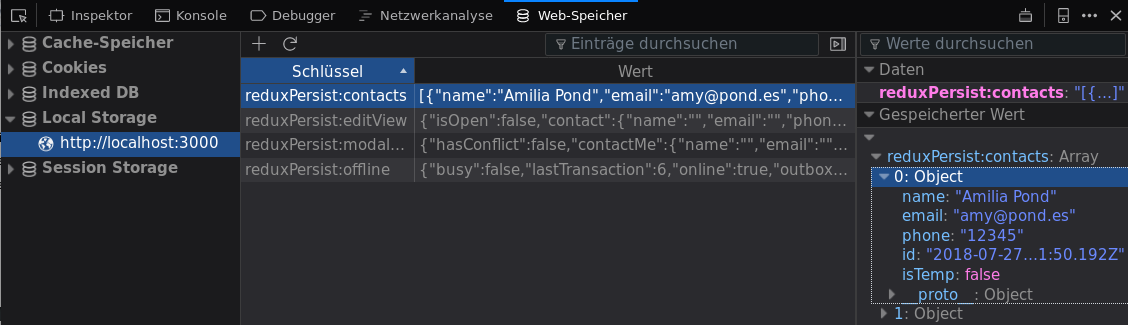
\includegraphics[width=\textwidth]{impl/localRdx}
  \grayRule
  \caption[Gespeicherte Daten im LocalStorage]{Gespeicherte Daten des Prototypen \it{amilia-rdx} im LocalStorage,\\Screenhot: Developer Tools im Firefox Browser}
  \label{fig:local-rdx}
\end{figure}
% 
Der Prototyp \it{amilia-qouch} nutzt zur lokalen Datenspeicherung PouchDB. PouchDB speichert die von NutzerInnen generierten Daten in IndexedDB, vgl. \autoref{chap:pouch}. In \autoref{fig:local-qouch} sind die gespeicherten Daten in der IndexedDB zu sehen.
%
\begin{figure}[H]
  \centering
  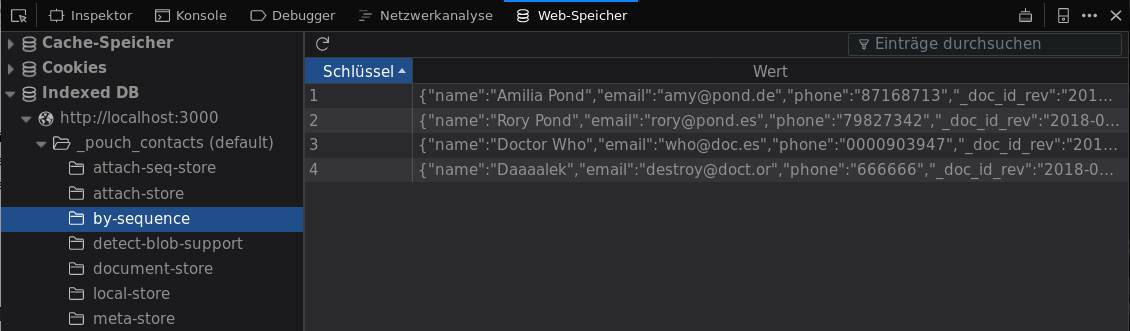
\includegraphics[width=\textwidth]{impl/localQouch}
  \grayRule
  \caption[Gespeicherte Daten in IndexedDB]{Gespeicherte Daten des Prototypen aus \it{amilia-qouch} in IndexedDB,\\Screenhot: Developer Tools im Firefox Browser}
  \label{fig:local-qouch}
\end{figure}
%
% SYNC
%
\sub{Datenbanksynchronisation}
Zwischen PouchDB und CouchDB können Daten in Echtzeit synchronisiert werden. Um die Live--Replikation zu aktivieren, muss im Synchronisationsaufruf der Parameter \tt{live: true} gesetzt sein.
Bricht die Internetverbindung ab, stoppt auch die Synchronisation.
Dank der angegebenen Parameter \tt{retry: true} versucht PouchDB die Synchronisation solange neuzustarten bis die Anwendung wieder mit dem Internet verbunden ist. \autoref{code:sync} zeigt die Implementation der Datenbankensynchronisation im Prototypen \it{amilia-qouch}.
%
\begin{center}
  \lstinputlisting[language=REACT,
  numbers=left,xleftmargin=20pt,
  firstline=1,lastline=5,
  framexleftmargin=15pt,
  caption={Synchronisation zwischen PouchDB und CouchDB im Prototyp \it{amilia-qouch}},
  label=code:sync]{code/sync.js}
\end{center}
Redux Offline nimmt einem auch Arbeit bei der Datensynchronisation ab. Alle Daten die sich im Queue befinden werden automatisch an den Server gesendet, sobald eine Internetverbindung besteht. Das funktioniert jedoch nicht so einfach wenn der Server nicht an ist. In der Dokumentation von Redux Offline steht, dass die Aktion solange versucht wird auszuführen, bis die Anwendung wieder mit dem Internet verbunden ist ~\cite{giving-up}. Allerdings wird die \sc{rollback} Aktion gefeuert wenn der Server nicht verfügbar ist und die Aktion wird abgebrochen.
\begin{center}
  \lstinputlisting[language=REACT,
  numbers=left,xleftmargin=20pt,
  firstline=6,
  framexleftmargin=15pt,
  caption={Discard Konfiguration für amilia-rdx},
  label=code:discard]{code/sync.js}
\end{center}
Die Discard Konfiguration bestimmt wann eine Aktion abgebrochen, und wann sie immer wieder neugestartet wird. Im \autoref{code:discard} ist in den Zeilen 1 bis 4 abzulesen wie diese Konfiguration überschrieben wird. Nun wird die Aktion nur abgebrochen wenn der Server verfügbar ist und einen \gls{HTTP} Status zwischen 400 und 500 zurückgibt.
In den darauffolgenden Zeilen wird die eigens implementierte Konfiguration mit der Standardkonfiguration von Redux Offline zusammengeführt wird.
Alle Daten werden nun auch nach einem Ausfall an den Server gesendet.\\
Im Gegensatz zum \it{amilia-qouch} Prototypen werden die Daten nur in eine Richtung automatisch gesendet. Es gibt keine Implementierung einer automatischen Replikation von den Daten auf dem Server zum lokalen Speicher.
%
%
%
\section{\label{chap:konfliktmanagement}Konfliktmanagement}
Konflikte werden in beiden Prototypen manuell erzeugt, wobei die Vorgehensweise identisch ist.
Wie ein Konflikt herbeigeführt werden kann, wird in \autoref{chap:konzept:test} beschrieben.
Durch das regelmäßige Anfragen an den Server wird ermittelt, ob sich die Anwendung im Onlinestatus befindet oder nicht.
Konflikte können erzeugt werden, wenn mindestens ein Gerät auf dem die Anwendung läuft, nicht mit dem Internet verbunden ist.
Die Anzeige des Netzwerkstatus im Header dient der Kontrolle über diesen Status.
Die folgenden Codeausschnitte illustrieren das Konfliktmanagement im Prototypen \it{amilia-qouch}.\\
Konflikte werden in CouchDB gespeichert, damit in der Anwendung entschieden werden kann wie damit umgegangen wird.
Im \autoref{code:conflicts} werden alle Kontakteinträge geladen.
Weil der Parameter in Zeile 3 als Option mitgegeben wird, sind Konfliktinformationen für jeden Kontakt verfügbar.
Gibt es unterschiedliche Versionen eines Kontaktes kommt er mit dem Attribut \tt{\_conflicts} beim Client an, und zwar in Form einer Liste aus allen korrelierenden Revisionsnummern.
In Zeile 7 wird der erste konfliktbehaftete Kontakt, der vom Server kommt, ermittelt.
Wenn es einen Konflikt gibt, wird die Funktion \tt{getConflictRevisions} in Zeile 10 aufgerufen.
%
\begin{center}
  \lstinputlisting[language=REACT,
    firstline=1,lastline=12,
    numbers=left,xleftmargin=20pt,framexleftmargin=15pt,
    caption={Das Laden von konfliktbehafteten Kontakten},
    label=code:conflicts]{code/conflicts.js}
\end{center}
%
\autoref{code:conflicts2} zeigt die Umsetzung der \tt{getConflictRevisions()}.
Hier wird die konkurrierende Version des Kontakts ermittelt.
Außerdem wird die Herkunft jeder Version festgestellt und das Öffnen eines Konfliktdialogs eingeleitet.\\
In Zeile 2 werden die Variablen \tt{contactMe} und \tt{contactYou} initialisiert.
Die erste repräsentiert die lokale Version, \tt{contactYou} steht für die Version die aus der CouchDB kommt.
In Zeile 4 wird überprüft, ob die übergebene Version des Kontakts mit der zuletzt bearbeiteten übereinstimmt.
Entsprechend werden die Variablen \tt{contactMe} und \tt{contactYou} befüllt.
Die übergebene Version ist die von CouchDB festgelegte gewinnende Revision.
Die andere, konkurrierende Version wird in Zeile 8, bzw. in Zeile 13 durch die Übergabe der Revisionsnummer im Parameter geladen.
Die ID ist bei beiden Versionen identisch.\\
%
Dann wird das Öffnen des Konfliktdialogs durch das Aktualisieren des \gls{App}status initialisiert.
Die beiden Kontaktversionen werden ebenfalls in den State geladen, um im Dialog korrekt angezeigt zu werden.
%
\begin{center}
  \lstinputlisting[language=REACT,
    firstline=14,lastline=38,
    numbers=left,xleftmargin=20pt,framexleftmargin=15pt,
    caption={Das Ermitteln von konkurrierenden Kontaktversionen},
    label=code:conflicts2]{code/conflicts.js}
\end{center}
%
Der Konfliktdialog ist in \autoref{fig:modal} dargestellt.
Im Titel steht der Name der lokalen Version, rot hervorgehoben.
Darunter befinden sich zwei große Knöpfe in unterschiedlichen Farben.
Der erste zeigt die Version des Kontakts, die vom Server kommt, die auf einem anderen Gerät bearbeitet wurde.
Der zweite, untere Knopf beinhaltet alle relevanten Informationen über die lokale Version des konfliktbehafteten Kontakts.
So ist zu erkennen welche der beiden Versionen die eigene ist und worin sie sich von der anderen unterscheidet.
%
\begin{figure}[H]
  \centering
  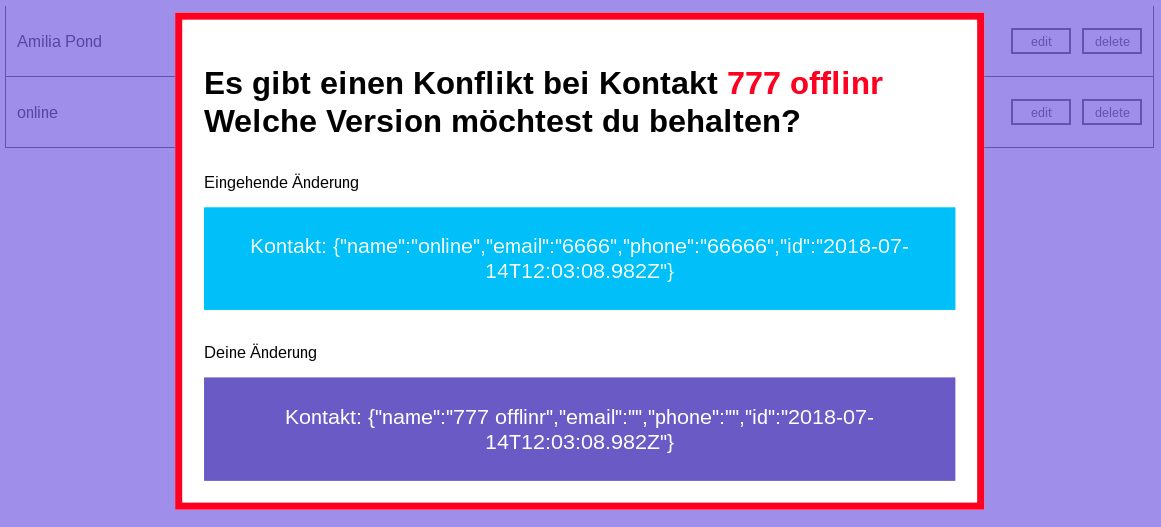
\includegraphics[width=\textwidth]{impl/Modal}
  \grayRule
  \caption{Konfliktdialog des Prototypen amilia-qouch}
  \label{fig:modal}
\end{figure}
%
Durch das Klicken einer dieser Knöpfe wird entschieden, welche der beiden Versionen behalten und welche eliminiert wird.
Wird der Knopf mit der lokalen Version betätigt, wird die in \autoref{code:conflicts3} gelistete Funktion \tt{removeRev} mit der anderen Version im Parameter aufgerufen.
%
\begin{center}
  \lstinputlisting[language=REACT,
    firstline=40,lastline=43,
    numbers=left,xleftmargin=20pt,framexleftmargin=15pt,
    caption={Das Eliminieren der verlierenden Version},
    label=code:conflicts3]{code/conflicts.js}
\end{center}
%
In Zeile 3 wird die verlierende Revision gelöscht.\\\\
%
%
Der Konfliktdialog konnte für den Protoypen \it{amilia-rdx} nicht umgesetzt werden, da Redux Offline nicht die Möglichkeit bietet Konflikte zu erkennen, geschweige denn zu speichern.
%
% Installationsanleitung
%
\section{Installationsanleitung}
\todo{build und so}
Beide entwickelten Prototypen sind als öffentliche Repositories auf GitHub\footnote{Software--Entwicklungs--Plattform \url{https://github.com/}} zu finden. 
Um sie zu installieren müssen folgende Schritte ausgeführt werden.
\sub{amilia-qouch}
1. Zuerst muss das Repository kopiert werden:
\lstset{language=sh, caption={},belowcaptionskip=0.3\baselineskip}
\begin{lstlisting}
git clone git@github.com:hulkoba/amilia-qouch.git
# oder
git clone https://github.com/hulkoba/amilia-qouch.git
\end{lstlisting}
2. Dann muss man in das Verzeichnis navigieren und alle Abhängigkeiten installieren.
\begin{lstlisting}
cd amilia-qouch
npm install
\end{lstlisting}
3. Mittels
\begin{lstlisting}
npm start
\end{lstlisting}
wird die Anwendung gestartet.
%
\sub{amilia-rdx}
1. Auch hier muss das Repository zuerst kopiert werden:
\lstset{language=sh, caption={},belowcaptionskip=0.3\baselineskip}
\begin{lstlisting}
git clone git@github.com:hulkoba/amilia-rdx.git
# oder
git clone https://github.com/hulkoba/amilia-rdx.git
\end{lstlisting}
2. Schritt zwei ist identisch mit dem in der \tt{amilia-qouch} Anleitung\\
3. Mittels
\begin{lstlisting}
npm run server
npm start
\end{lstlisting}
wird zuerst der Server, dann die Anwendung gestartet.

%
% Testfälle
%
\section{\label{chap:impl:test}Testfälle}
\section{\label{sec:impl:test}Testfälle}
Folgende Testfälle zur Offlinefunktionalität werden während der Entwicklung stetig durchgeführt. Das erfolgreiche Bestehen dieser Tests ist eine notwendige Qualitätseigenschaft der zu entwickelnden Prototypen.
\begin{description}[leftmargin=0.7cm,style=nextline]
\item[Netzwerkstatus:] 
Die Anwendung muss zu jeder Zeit den korrekten Netzwerkstatus anzeigen.\\
\item[Kontakte lesen:] 
Die Anwendung bei jedem Start die Kontakte aus dem lokalen Speicher oder aus der \it{Datenbank} laden.\\
\item[Kontakt anlegen:] 
Die Anwendung muss zu jedem Zeitpunkt in der Lage sein einen Kontakt mit jedem seiner Attribute anzulegen. Dazu muss er immer lokal gespeichert werden und sobald eine Internetverbindung besteht, persistiert werden.
Das Anlegen eines Kontakts im Offlinestatus ist für die Konfliktforcierung erforderlich.\\
\item[Kontakt bearbeiten:] 
Die Anwendung muss zu jedem Zeitpunkt in der Lage sein einen Kontakt mit jedem seiner Attribute zu bearbeiten. Ist keine Internetverbindung vorhanden, müssen die Änderungen lokal übernommen und später, sobald sich der Netzwerkstatus ändert, synchronisiert werden.
Das Bearbeiten eines Kontakts im Offlinestatus ist für die Konfliktforcierung erforderlich.\\
\item[Kontakt löschen:] 
Die Anwendung muss zu jedem Zeitpunkt in der Lage sein einen Kontakt zu löschen.
Das Löschen eines Kontakts im Offlinestatus ist für die Konfliktforcierung erforderlich.
\end{description}